\subsection{Correction method}

After plotting the radiant intensity for each region of interest it is apparent that there are unnatural jumps within the signal (\ref{fig:raw15}). Those jumps occur in each region of interest at the same time and are shown by a high difference of the values between two frames. The amount of the observed jumps varies between 0 and 20 in the recordings. Furthermore the appearance of the jumps is non-periodic and in each recording at different time points.
\begin{figure}[H]
	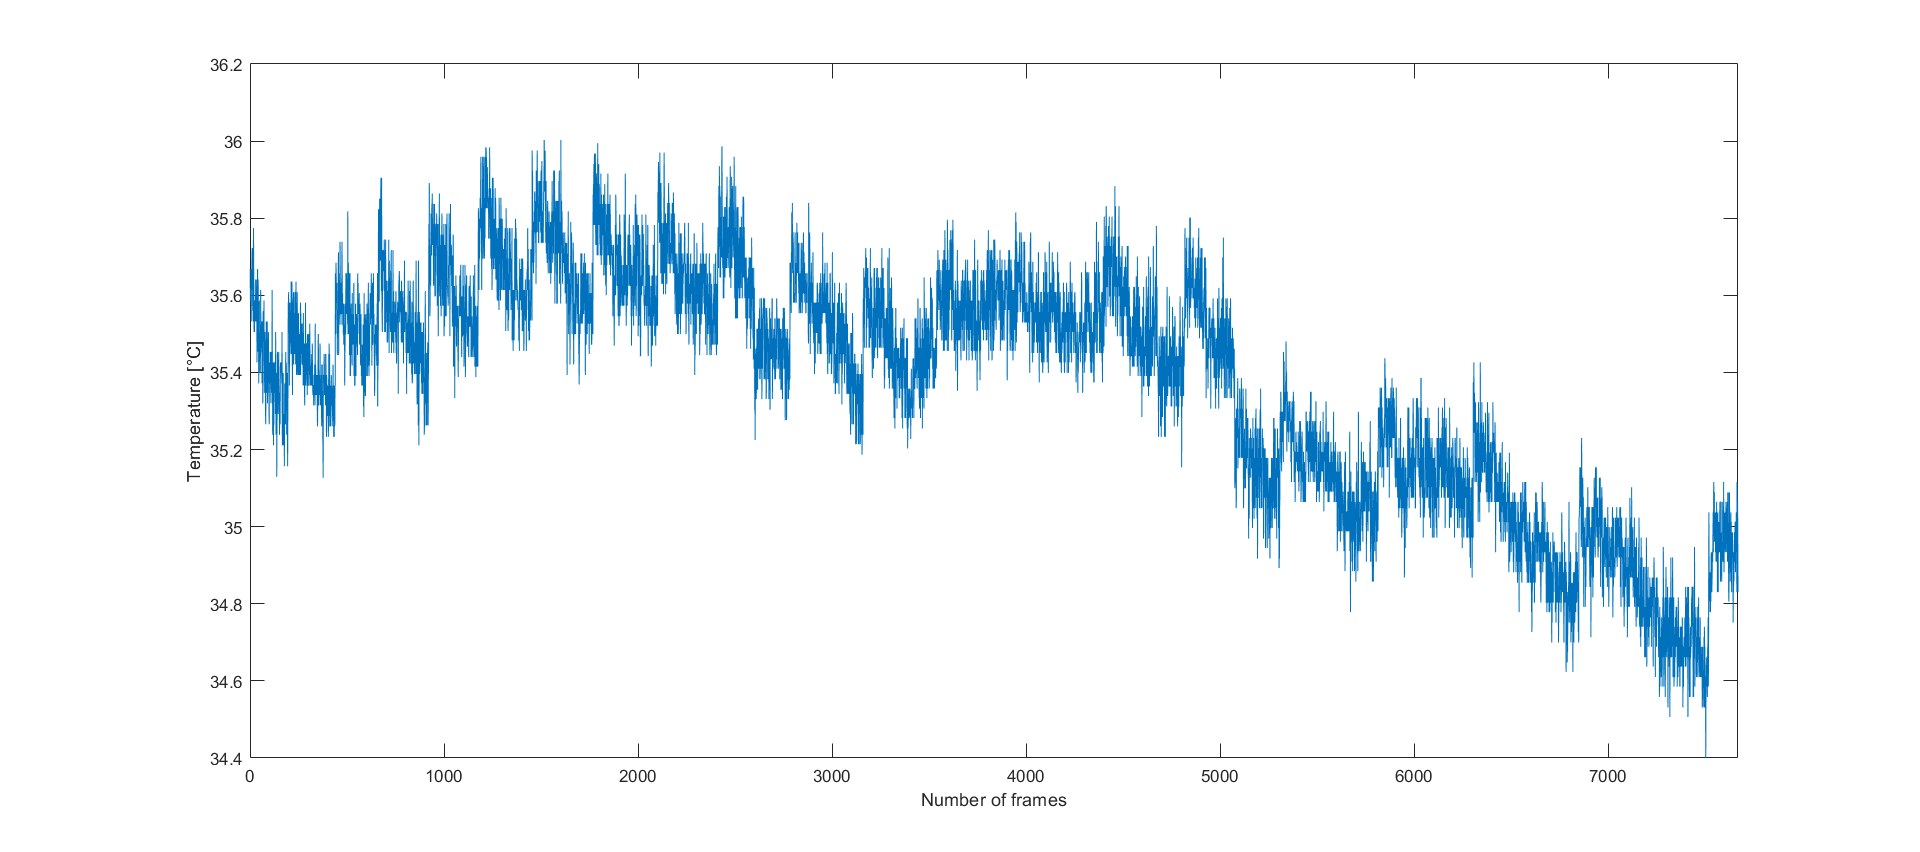
\includegraphics[width=0.6\textwidth]{figures/raw15}
	\caption{The original data of region 15 in the uncuffed recording of subject 1 including 20 jumps.}
	\label{fig:raw15}
\end{figure}
A continuous wavelet transform out of the raw data shows a magnitude scalogram with high magnitude peaks exactly at the same time points where the jumps are occurring. Due to this falsifying of the magnitude, the results of the data analysis are also falsified.
Additionally there is also a drift occurring within each interval between two jumps, which hampers the correct data analysis. To reduce the drift component and the jumps in the signals, the two following correction methods have been implemented.

\textbf{Method 1: Regression of first interval}
The first implemented method is based on the assumption that the drift is equal in each interval. It is also assumed that the camera has been calibrated just before the recording, so the first interval can be used as a reference to calculate the drift component. Therefore a linear regression for the first interval has been made. With the resultant slope $m$ follows the calculation of the drift difference $d$ within the first interval. Due to the assumption, that the drift difference is equal, the slope of the drift of each interval depends on the length of the interval. The slopes have been calculated with the equation $m=\frac{d}{length(interval)}$.
To compensate the drift, a straight with the inverse slope and the starting point in the first data point of the interval has been calculated. The middle points between the original data and the new calculated straight build the correction of the data signal.
This correction worked within the signal just in several parts and had a lot of weak points where the jumps have been strengthened. Due to the outcome of this method the assumption, that the drift is equal in each interval has been discarded. 


\textbf{Method 2: Regression of each interval}
The second implemented method is due to the failure of the first method based on the assumption that the drift is not equal in each interval. Out of the recorded data the exact drift is indeterminable. Hence a method which tries to fit the separate intervals together without the necessity of the awareness of the real drift component and avoids the suppression of the basic shape of the signal has been chosen.
Therefore firstly the linear regressions for all intervals and the corresponding residuals are calculated.
The idea is to move the end point of a regression line and the start point of the next regression line together. Thus the middle points between end and following start point are calculated. The alignment of the regression lines is changed, so that the start and end points of all the new created orientation straights fit the middle points, except the first and the last orientation straight. Both fit just one middle point. For the start of the first orientation straight is the start point of the regression line of the first interval and for the end point of the last orientation straight is the end point of the regression line of the last interval used.
\begin{figure}[H]
	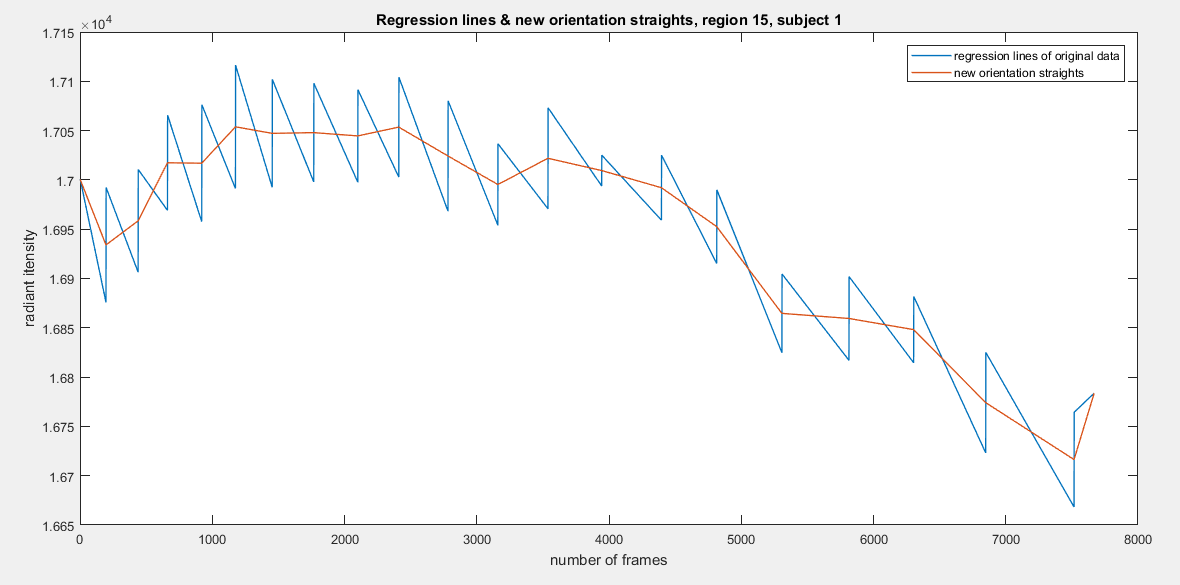
\includegraphics[width=0.6\textwidth]{figures/reg15}
	\caption{Connected regression lines of the original data of region 15 in the uncuffed recording of subject 1 in blue. New created orientation line of the same recording in the same region shown in red.}
	\label{fig:reg15}
\end{figure}
As shown in \ref{fig:reg15} the new orientation straight fits the regression lines together without suppressing the shape of the signal. Subsequently the residuals have been added to the new orientation straight, to sustain the ratio between the data points. \ref{fig:corr15} shows the corrected signal wherein the with jumps separated intervals have been connected and the jumps have been largely corrected.
\begin{figure}[H]
	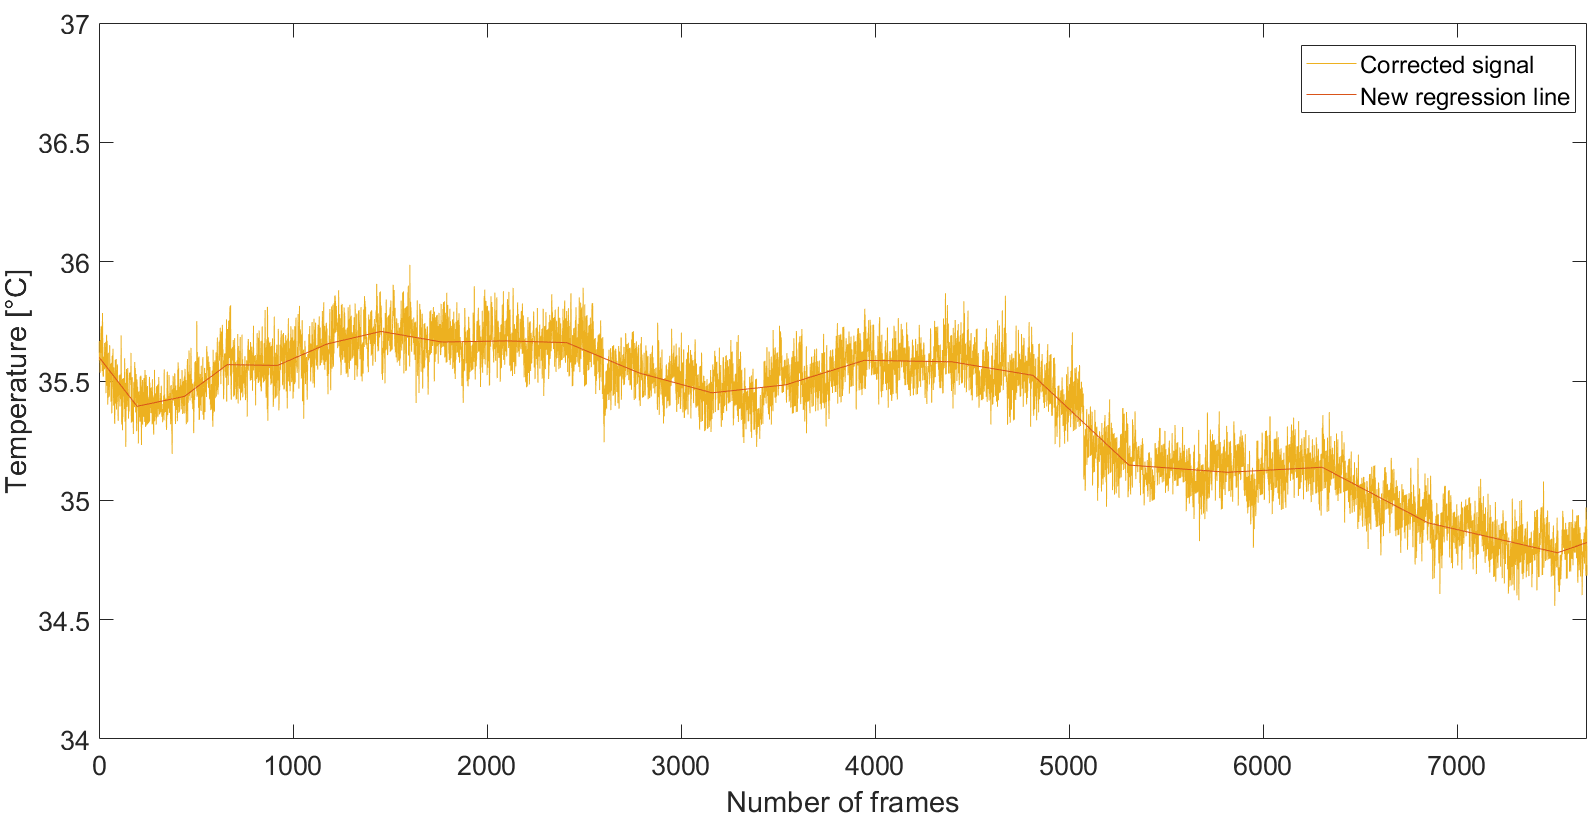
\includegraphics[width=0.6\textwidth]{figures/corr15}
	\caption{Orientation line based on the data of the uncuffed recording of subject 1 in region 15 shown in red. Corrected signal of the same data in yellow.}
	\label{fig:corr15}
\end{figure}
However, this method has still weak points. The shown region of interest is located in the center of the thermal image. Regions which are located in the outer area of the thermal image show after the correction a few jumps which are bigger than before (\ref{fig:corr23}). These sporadic extended jumps are due to the fact that the thermal image is more unstable in the outer areas than in the center, thus the pixel drift is increasing with increasing distance of the center.
\begin{figure}[H]
	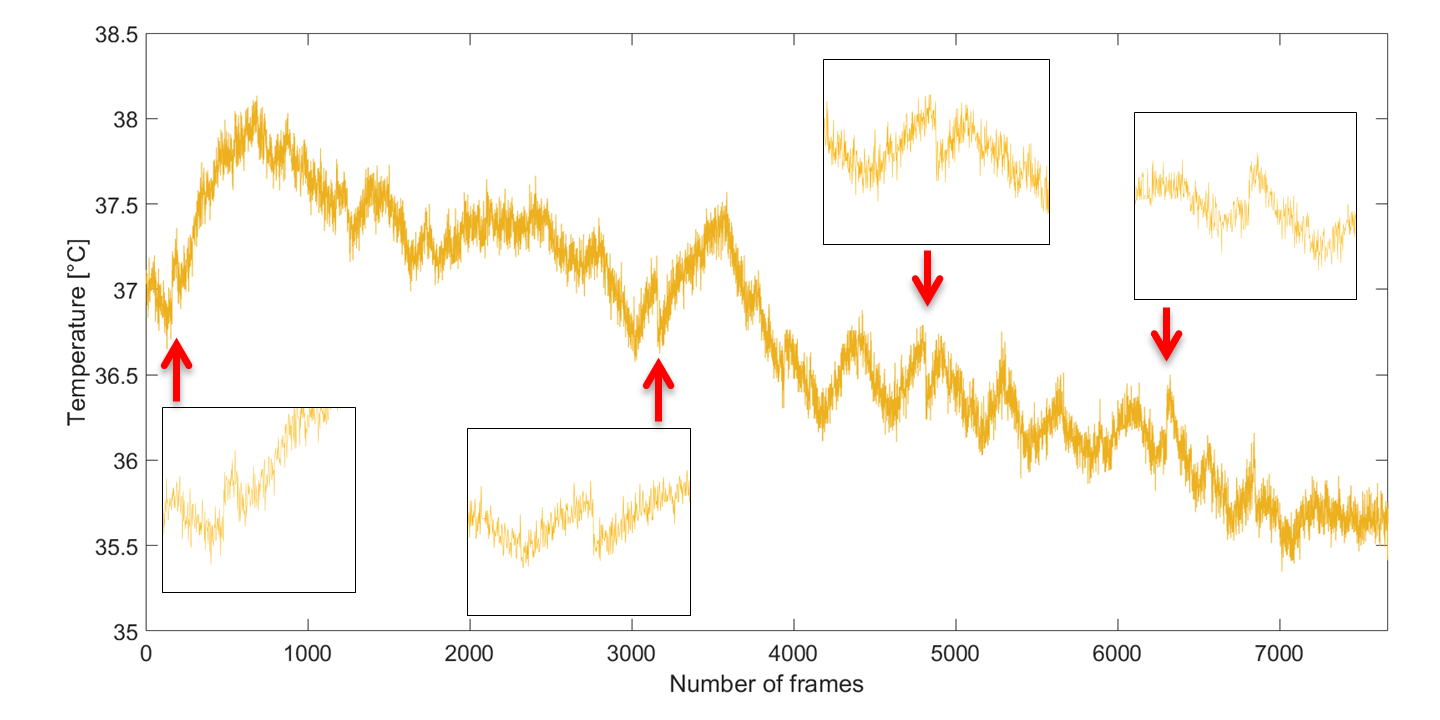
\includegraphics[width=0.6\textwidth]{figures/corr23pfeile}
	\caption{Corrected data of the uncuffed recording of subject 1 in region 23 shown in yellow. Red arrows show the jumps in this signal.}
	\label{fig:corr23}
\end{figure}